\AUTChapter{Introduction} \label{chap:intro}
\section{Introduction}
\nobreak
This is the introduction chapter. \marginNote{This is an example of a margin note, say to highlight something for your supervisor to look at} Note that the chapter titles are noted as \texttt{myChapter}. Read the class file to see how sample chapters can be printed. For the marginal note, use the command 
\begin{verbatim}
\marginNote{...}
\end{verbatim}

%\begin{comment}
This is an example of a cross reference to a figure, Fig.~\ref{fig:intro:graphSample} on page \pageref{fig:intro:graphSample}, however using the package varioref, we get Fig.~		\vref{fig:intro:graphSample}.
%\end{comment}

\begin{figure}[ht] %  figure placement: here, top, bottom, or page
   \centering
   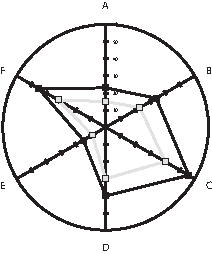
\includegraphics[width=0.3\linewidth]{graphSample} 
   \caption[Sample image]{This is a sample image file}
   \label{fig:intro:graphSample}
\end{figure}

\newpage{}
\section{Table styles}

\begin{table}[ht]
	\caption[Principle-Based Method of Systems Analysis]{Principle-Based Method of Systems Analysis Method \emph{\protect\cite{Alter2002}}} \label{tab:pbmsa}
	\centering\RaggedRight
	\begin{tabular}[t]{p{4cm}p{9cm}}
	\toprule
	\textbf{Systems analysis step} & \textbf{Steps in \textsc{pbmsa}} \\
	\hline
	1. Define the problem & Define the problem and Work System together \\
	\hline
	\parbox[t]{\linewidth}{2. Design potential improvements} & \parbox[t]{\linewidth}{Use each Work Principle in turn as a lens for summarising the current situation and search for possible improvements. 
	\begin{description} 
	\item[Principle 1] Please the Customers
	\item[Principle 2] Perform the work efficiently
	\item[Principle 3] Serve the Participants
	\item[Principle 4] Create value from information
	\item[Principle 5] Minimise effort absorbed by technology
	\item[Principle 6] Take full advantage of infrastructure
	\item[Principle 7] Minimise unintended conflicts and risks
	\item[Principle 8] Support organisational strategy
	\item[Principle 9] Maintain balance between Work System elements
	\end{description}}\\ 
	\hline
	3. Decide what to do & Make a recommendation that addresses the problem while supporting the organisation's priorities. \\
	\bottomrule
	\end{tabular}
\end{table}

This is a link to Fig.~\vref{fig:intro:graphSample}.

\singlespacing
\begin{longtable}[t]{c p{6cm} l}
\caption[Extended version of Work System Principles]{Extended version of Work System Principles \\ \indent{}\emph{Source: \protect\cite<Adapted from>[Table 2, pp.~1607--8]{Alter2004}} \label{tab:ExtendedWSPrinciples}}\\
\toprule
& \textbf{Work system principle} & \textbf{Related Work System element}\\
\hline
\endfirsthead

\caption[]{Extended version\dots{} \emph{(continued)}}\\
\toprule
& \textbf{Work system principle} & \textbf{Related Work System element}\\
\hline
\endhead

\hline
& & \hfill\emph{Continued over page} \\
\bottomrule
\endfoot

\bottomrule
\endlastfoot

& \textbf{1:} Please the customers. & Customers and products \& services \\
\dag{}\footnote{Those principles that have been added in Alter's revision are indicated with a \dag{} symbol.} & \textbf{2:} Balance priorities of different customers. & Customers and products \\
\dag{} & \textbf{3:} Match process flexibility with product variability. & Product and work practices\footnote{Previously referred to as Business Processes, Alter has changed term to ``work practices.''} \\
& \textbf{4:} Perform the work efficiently. & Work practices \\
\dag{} & \textbf{5:} Encourage appropriate use of judgement. & Work practices \\
\dag{} & \textbf{6:} Control variances (problems) at their source. & Work practices \\
\dag{} & \textbf{7:} Monitor the quality of both inputs and outputs. & Work practices \\
\dag{} & \textbf{8:} Boundaries between business process steps should facilitate control & Work practices \\
\dag{} & \textbf{9:} Match the work practices with the participants. & Work practices and participants \\
& \textbf{10:} Serve the participants & Participants \\
\dag{} & \textbf{11:} Align participant incentives with system goals & Participants \\
\dag{} & \textbf{12:} Provide information where it will affect action & Information and work practices \\
\dag{} & \textbf{13:} Protect information from inappropriate use & Information \\
\dag{} & \textbf{14:} Use appropriate technology & Technology and work practices \\
& \textbf{15:} Minimise effort consumed by technology & Technology \\
& \textbf{16:} Take full advantage of infrastructure & Infrastructure \\
& \textbf{17:} Minimise unnecessary conflict with the external environment & Environment\footnote{Previously referred to as Context, Environment is distinct from Infrastructure and Technology whereas Context could be confused with both.} \\
& \textbf{18:} Support the firm's strategy & Strategy \\
& \textbf{19:} Minimise unnecessary risks & System as a whole \\
& \textbf{20:} Maintain balance between work system elements & System as a whole \\
\dag{} & \textbf{21:} Maintain the ability to adapt, change, and grow. & System as a whole \\
\end{longtable}
\doublespacing

A sample citation: \cite{Bannon1997}.

apacite specific examples:
\begin{itemize} 
\item \citeA{Bannon1997}
\item \citeNP{Bannon1997}
\end{itemize}

\newpage{}
\section{Listing styles}
\subsection{Itemised list}
This listing style uses \texttt{itemize*} to pull the increased line spacing closer.
\begin{itemize*}
\item Lorem ipsum dolor sit amet, consetetur sadipscing elitr, sed diam nonumy eirmod tempor invidunt ut labore et dolore magna aliquyam erat, sed diam voluptua. '
\item At vero eos et accusam et justo duo dolores et ea rebum. 
\item Stet clita kasd gubergren, no sea takimata sanctus est Lorem ipsum dolor sit amet. Lorem ipsum dolor sit amet, consetetur sadipscing elitr, sed diam nonumy eirmod tempor invidunt ut labore et dolore magna aliquyam erat, sed diam voluptua.
\end{itemize*}

\subsection{Enumerated list}
This listing style uses \texttt{enumerate*} to pull the increased line spacing closer.
\begin{enumerate*}
\item Lorem ipsum dolor sit amet, consetetur sadipscing elitr, sed diam nonumy eirmod tempor invidunt ut labore et dolore magna aliquyam erat, sed diam voluptua. '
	\begin{enumerate*}
	\item Lorem ipsum dolor sit amet, consetetur sadipscing elitr, sed diam nonumy eirmod tempor invidunt ut labore et dolore magna aliquyam erat, sed diam voluptua. '
	\item At vero eos et accusam et justo duo dolores et ea rebum. 
	\item Stet clita kasd gubergren, no sea takimata sanctus est Lorem ipsum dolor sit amet. Lorem ipsum dolor sit amet, consetetur sadipscing elitr, sed diam nonumy eirmod tempor invidunt ut labore et dolore magna aliquyam erat, sed diam voluptua.
	\end{enumerate*}
\item At vero eos et accusam et justo duo dolores et ea rebum. 
\item Stet clita kasd gubergren, no sea takimata sanctus est Lorem ipsum dolor sit amet. Lorem ipsum dolor sit amet, consetetur sadipscing elitr, sed diam nonumy eirmod tempor invidunt ut labore et dolore magna aliquyam erat, sed diam voluptua.
\end{enumerate*}

\subsection{Description list}
This listing style uses \texttt{description*} to pull the increased line spacing closer.
\begin{description*}
\item[Lorem ipsum] dolor sit amet, consetetur sadipscing elitr, sed diam nonumy eirmod tempor invidunt ut labore et dolore magna aliquyam erat, sed diam voluptua. '
	\begin{enumerate*}
	\item Lorem ipsum dolor sit amet, consetetur sadipscing elitr, sed diam nonumy eirmod tempor invidunt ut labore et dolore magna aliquyam erat, sed diam voluptua. '
	\item At vero eos et accusam et justo duo dolores et ea rebum. 
	\item Stet clita kasd gubergren, no sea takimata sanctus est Lorem ipsum dolor sit amet. Lorem ipsum dolor sit amet, consetetur sadipscing elitr, sed diam nonumy eirmod tempor invidunt ut labore et dolore magna aliquyam erat, sed diam voluptua.
	\end{enumerate*}
\item[At vero eos et accusam] et justo duo dolores et ea rebum. 
\item[Stet clita kasd gubergren] no sea takimata sanctus est Lorem ipsum dolor sit amet. Lorem ipsum dolor sit amet, consetetur sadipscing elitr, sed diam nonumy eirmod tempor invidunt ut labore et dolore magna aliquyam erat, sed diam voluptua.
\end{description*}

\section{Some various citation styles}
\nobreak
Lorem ipsum dolor sit amet, consetetur sadipscing elitr, sed diam nonumy eirmod tempor invidunt ut labore et dolore magna aliquyam erat, sed diam voluptua \cite{Quine2004}. At vero eos et accusam et justo duo dolores et ea rebum. Stet clita kasd gubergren, no sea takimata sanctus est Lorem ipsum dolor sit amet \cite{Peirce1992a}. Lorem ipsum dolor sit amet, consetetur sadipscing elitr, sed diam nonumy eirmod tempor invidunt ut labore et dolore magna aliquyam erat, sed diam voluptua.

 duis autem vel eum iriure dolor in hendrerit in vulputate velit esse molestie consequat, ``vel illum dolore eu feugiat nulla facilisis at vero eros et accumsan et iusto odio dignissim qui blandit praesent luptatum zzril delenit augue duis dolore te feugait nulla facilisi'.

\section{Some verbatim code}

\begin{verbatim}
this is some code
    this code is indented
        and further indented
\end{verbatim}
\section{Conclusion}
\nobreak
Lorem ipsum dolor sit amet, consetetur sadipscing elitr, sed diam nonumy eirmod tempor invidunt ut labore et dolore magna aliquyam erat, sed diam voluptua. At vero eos et accusam et justo duo dolores et ea rebum. Stet clita kasd gubergren, no sea takimata sanctus est Lorem ipsum dolor sit amet. Lorem ipsum dolor sit amet, consetetur sadipscing elitr, sed diam nonumy eirmod tempor invidunt ut labore et dolore magna aliquyam erat, sed diam voluptua.

Duis autem vel eum iriure dolor in hendrerit in vulputate velit esse molestie consequat, vel illum dolore eu feugiat nulla facilisis at vero eros et accumsan et iusto odio dignissim qui blandit praesent luptatum zzril delenit augue duis dolore te feugait nulla facilisi.

Lorem ipsum dolor sit amet, consetetur sadipscing elitr, sed diam nonumy eirmod tempor invidunt ut labore et dolore magna aliquyam erat, sed diam voluptua. At vero eos et accusam et justo duo dolores et ea rebum. Stet clita kasd gubergren, no sea takimata sanctus est Lorem ipsum dolor sit amet. Lorem ipsum dolor sit amet, consetetur sadipscing elitr, sed diam nonumy eirmod tempor invidunt ut labore et dolore magna aliquyam erat, sed diam voluptua.

Duis autem vel eum iriure dolor in hendrerit in vulputate velit esse molestie consequat, vel illum dolore eu feugiat nulla facilisis at vero eros et accumsan et iusto odio dignissim qui blandit praesent luptatum zzril delenit augue duis dolore te feugait nulla facilisi.

Lorem ipsum dolor sit amet, consetetur sadipscing elitr, sed diam nonumy eirmod tempor invidunt ut labore et dolore magna aliquyam erat, sed diam voluptua. At vero eos et accusam et justo duo dolores et ea rebum. Stet clita kasd gubergren, no sea takimata sanctus est Lorem ipsum dolor sit amet. Lorem ipsum dolor sit amet, consetetur sadipscing elitr, sed diam nonumy eirmod tempor invidunt ut labore et dolore magna aliquyam erat, sed diam voluptua.

Duis autem vel eum iriure dolor in hendrerit in vulputate velit esse molestie consequat, vel illum dolore eu feugiat nulla facilisis at vero eros et accumsan et iusto odio dignissim qui blandit praesent luptatum zzril delenit augue duis dolore te feugait nulla facilisi.